\documentclass[a4paper,10pt,twocolumn]{ltjsarticle}
\usepackage[haranoaji]{luatexja-preset}
\usepackage[top=18mm,bottom=20mm,left=17mm,right=17mm,columnsep=8mm]{geometry}
\usepackage{graphicx,booktabs,array,caption,enumitem,xcolor,tikz}
\usetikzlibrary{shapes.geometric}
\setlength{\parindent}{1\zw}
\renewcommand{\baselinestretch}{1.0}
\setlength{\parskip}{0pt}
\renewcommand{\thesection}{\arabic{section}.}
\renewcommand{\thesubsection}{\arabic{section}.\arabic{subsection}.}
\makeatletter
\renewcommand{\section}{\@startsection{section}{1}{\z@}{1.1\Cvs \@plus.4\Cdp \@minus.2\Cdp}{.5\Cvs \@plus.2\Cdp}{\normalfont\gtfamily\bfseries\large}}
\renewcommand{\subsection}{\@startsection{subsection}{2}{\z@}{.8\Cvs \@plus.3\Cdp \@minus.2\Cdp}{.3\Cvs \@plus.1\Cdp}{\normalfont\gtfamily\bfseries\normalsize}}
\makeatother
\captionsetup{font={small,sf},labelsep=space,justification=raggedright,singlelinecheck=false,skip=3pt}
\captionsetup[table]{position=top}
\setlist[itemize]{leftmargin=1.2\zw,itemsep=0pt,topsep=2pt,parsep=0pt}
\setlength{\textfloatsep}{8pt plus 2pt minus 2pt}
\setlength{\floatsep}{8pt plus 2pt minus 2pt}
\setlength{\intextsep}{8pt plus 2pt minus 2pt}
\pagestyle{plain}
\raggedbottom
\begin{document}
\twocolumn[{
\noindent\fbox{\gtfamily\small\ 生成AI論文\ }\par\medskip
\begin{center}
{\gtfamily\bfseries\LARGE 日本の大人は，プログラミングや表計算をどれだけしているのか：UNESCOのデータで47の国・地域と比べる$^{\dagger}$}\par\medskip
{\gtfamily\bfseries\large プログラミング・表計算・プレゼン資料作成の割合と国・地域間の関連}\par\medskip
{\normalsize EduData調査研究グループ$^{*1}$・教育データサイエンス解析班$^{*2}$}\par
{\small オープン教育統計推進プロジェクト$^{*1}$・初等中等STEM教育データ基盤ユニット$^{*2}$}
\end{center}\smallskip
\noindent\begin{minipage}{\textwidth}\small UNESCO統計研究所の2021年公表値（元はITU）を用い，プログラミング，表計算ソフトの算術式，プレゼン資料作成を「した」成人の割合を47の国・地域で比べた．日本は，プログラミング5.6\%（平均6.31\%，21番目，スロベニアと同値），表計算50.9\%（平均34.31\%，7番目），プレゼン資料作成33.5\%（平均29.75\%，21番目）であった．平均は国・地域を同じ重みで扱った単純平均である．表計算の割合が高い国・地域ほどプログラミングの割合も高く（\textit{r}=.79，95\%CI [0.65, 0.88]，\textit{ρ}=.76，\textit{n}=47，\textit{p}<.001，\textit{BF}\textsubscript{10}>1000），サウジアラビアとアラブ首長国連邦を除いても \textit{r}=.70であった．日本は表計算から見込まれるよりプログラミングが低かった．ただしプレゼン資料作成との相関（\textit{r}=.77）と差は示せず，重回帰では表計算の係数の信頼区間が0を含んだ．結果は国・地域の集計値の記述であり，個々の成人の因果や理由は示さない．\par\smallskip
\noindent{\gtfamily キーワード：}UNESCO，ICTスキル，国際比較，プログラミング，表計算\end{minipage}\medskip
}]
\let\thefootnote\relax
\footnotetext{\footnotesize 2026年10月執筆\\ $^{\dagger}$How Much Do Adults in Japan Use Programming and Spreadsheets? Comparing Japan with 47 Countries and Regions using UNESCO Data†\\ $^{*1}$ Open Education Data Project, Tokyo, Japan\quad $^{*2}$ Educational Data Science Unit, Tokyo, Japan}
\section{はじめに}
\subsection{研究の背景}
プログラミングや表計算などの情報活用の行動は，教育や仕事の基盤として注目されている．Wing (2006)は計算論的思考を論じ，Ragnedda (2018)はデジタル資本の概念を整理した．デジタル格差については，Selwyn (2004)が政治や世間での捉え方を問い直し，Hargittai (2002)は利用者のオンラインスキルの違いに注目し，Van Deursen and Van Dijk (2014)は格差が利用の違いへ移ることを論じ，Van Dijk (2020)はデジタル格差を一冊で論じている．ITU (2023)は世界のデジタル化の指標と数値を公表し，UNESCO (2023)は教育でのテクノロジーが誰の条件で使われるのかを問うた．

本研究は，UNESCO統計研究所のSDG 4.4.1データ（元はITUが各国の調査から集めた統計）を用い，3つの活動の割合の国・地域間の分布と日本の位置，および表計算とプログラミングの国・地域間の関連を記述する．両者は同じ機器や回線，学ぶ機会を必要とするので，国・地域間で並んで高くなると予想するが，これは仮説である．
\subsection{リサーチクエスチョン}
本研究の目的は，プログラミング，表計算，プレゼン資料作成を「した」成人の割合の国・地域間分布と日本の位置を記述し，表計算とプログラミングの国・地域間の関連を調べることである．
\begin{itemize}
\item RQ1：プログラミング・表計算・プレゼン資料作成をした人の割合は，国・地域によってどう違い，日本はどこに位置するか．
\item RQ2：表計算ソフトで算術式を使った人の割合が高い国・地域ほど，プログラミングをした人の割合も高いか（国・地域間の関連として）．
\end{itemize}
\section{調査対象および分析方法}
UNESCO統計研究所の2021年公表値から，3つの総計の指標がそろう47の国・地域を取り込んだ．分析単位は国・地域で，各国・地域を同じ重みで扱ったため，平均や中央値は成人の人数で重みづけした値ではない．順位は，大きい値から数え，同じ値は同順位とした．

相関はピアソンの \textit{r}，95\%信頼区間，スピアマンの \textit{ρ}，\textit{p}，JZSベイズファクター \textit{BF}\textsubscript{10}（尺度1）で示し，\textit{BF}\textsubscript{10}が3を超えれば関連を支持，1/3未満なら関連がないことを支持とみなした．全ペアの探索は42組で，多重比較の基準は.05÷42（約.0012）である．男女計と男女別，男女差のように計算でつながる組は結果として解釈せず，RQ2に関わる組だけを報告した．比較として，プレゼン資料作成との相関と表計算の男女差との相関も示した．3つの割合の分母（全成人か利用者か），期間，日本の値の年齢範囲は，公表資料で確認できていない．

重回帰（\textit{n}=38）は，プログラミングの割合を目的変数，表計算・プレゼン資料作成・表計算の男女差を説明変数とし，標準化係数 \textit{β}，ブートストラップ（2000回）の95\%CI，\textit{p}，VIF，\textit{R}²，調整済み \textit{R}²を求めた．パス解析（\textit{n}=47）は表計算→プレゼン資料作成→プログラミングの経路で，直接・間接・総合の関連と間接の95\%CIを求めた．SEMは（\textit{n}=36），表計算とプレゼンの女性・男性別の4つの値を潜在変数にまとめ，プログラミングとの関連を見た．パス解析の向きは仮定で，3変数の飽和モデルは向きを入れ替えても同じ適合になる．特定の国・地域に依存しないかは，日本，上位2か国，1か国ずつを除いて確かめた．
\begin{table*}[!t]
\caption{主要指標の基本記述統計量}
\centering\small
\begin{tabular}{>{\raggedright\arraybackslash}p{9.2cm}rrrrrr}
\toprule
指標 & \textit{K} & 平均 & \textit{SD} & 中央値 & 最小 & 最大 \\
\midrule
プログラミングをした人の割合 & 47 & 6.3 & 5.3 & 5.2 & 0.6 & 25.2 \\
プログラミングをした女性の割合 & 36 & 5.1 & 5.9 & 3.0 & 0.4 & 24.7 \\
プログラミングをした男性の割合 & 36 & 8.8 & 6.1 & 7.8 & 0.7 & 25.6 \\
表計算ソフトで基本的な算術式を使った人の割合 & 47 & 34.3 & 18.0 & 36.8 & 3.6 & 84.4 \\
表計算で算術式を使った女性の割合 & 39 & 32.1 & 16.6 & 34.9 & 2.6 & 80.4 \\
表計算で算術式を使った男性の割合 & 38 & 37.6 & 19.1 & 38.9 & 4.5 & 85.9 \\
プレゼンテーション資料を作成した人の割合 & 47 & 29.8 & 16.5 & 31.1 & 1.0 & 61.7 \\
プレゼン資料を作成した女性の割合 & 39 & 27.6 & 16.2 & 29.1 & 0.8 & 63.0 \\
プレゼン資料を作成した男性の割合 & 38 & 30.4 & 17.8 & 29.6 & 1.3 & 64.0 \\
表計算の男女差（男性−女性，\%ポイント） & 38 & 5.0 & 5.8 & 3.6 & -4.1 & 18.8 \\
プレゼン資料作成の男女差（男性−女性，\%ポイント） & 38 & 2.3 & 5.5 & 2.0 & -14.9 & 17.4 \\
\bottomrule
\end{tabular}
\par\smallskip{\footnotesize 注）単位は\%，\textit{K}は観測数（国・地域・区分）．}
\end{table*}
\begin{table*}[!t]
\caption{主要指標間のピアソンの相関係数と，ベイズファクター}
\centering\small
\begin{tabular}{>{\raggedright\arraybackslash}p{6.4cm}>{\raggedright\arraybackslash}p{6.4cm}rrr}
\toprule
指標 \textit{X} & 指標 \textit{Y} & \textit{r} & \textit{p} & \textit{BF}\textsubscript{10} \\
\midrule
プログラミングをした人の割合 & 表計算ソフトで基本的な算術式を使った人の割合 & .79 & < .001 & >1000 \\
プログラミングをした人の割合 & プログラミングをした女性の割合 & .97 & < .001 & >1000 \\
プログラミングをした人の割合 & プログラミングをした男性の割合 & .97 & < .001 & >1000 \\
プログラミングをした人の割合 & 表計算で算術式を使った女性の割合 & .79 & < .001 & >1000 \\
プログラミングをした人の割合 & 表計算で算術式を使った男性の割合 & .77 & < .001 & >1000 \\
\bottomrule
\end{tabular}
\par\smallskip{\footnotesize 注）\textit{BF}\textsubscript{10}はJZSベイズファクター（3を超えれば関連を支持，1/3を下回れば関連がないことを支持）．全ペアの探索の一部を載せた．}
\end{table*}
\section{結果}
47の国・地域（表1）で，プログラミングをした人の割合は0.6\%（バングラデシュ）から25.2\%（サウジアラビア）に分布し，平均6.31\%，中央値5.2\%であった．日本は5.6\%で，これより高い国・地域は20，同じ値がスロベニアにあるため，公表値の順では21番目（スロベニアと同順位）である．平均よりやや低く，中央値よりやや高い．表計算で基本的な算術式を使った人の割合は3.6\%（イラン）から84.4\%（アラブ首長国連邦）に分布し（平均34.31\%，中央値36.8\%），日本は50.9\%で，これより高い国・地域は6，順位は7番目であった．プレゼン資料を作成した人の割合は1.0\%（バングラデシュ）から61.7\%（サウジアラビア）に分布し（平均29.75\%，中央値31.1\%），日本は33.5\%で，これより高い国・地域は20，順位は21番目であった．

RQ2について，プログラミングと表計算の相関は \textit{r}=.79（95\%CI [0.65, 0.88]，\textit{ρ}=.76，\textit{n}=47，\textit{p}<.001，\textit{BF}\textsubscript{10}>1000，表2）で，関連を支持した．プレゼン資料作成との相関も \textit{r}=.77（95\%CI [0.62, 0.87]，\textit{ρ}=.83，\textit{n}=47，\textit{p}<.001，\textit{BF}\textsubscript{10}>1000）で，2つの相関の差は示せなかった（Williamsのt=0.52，\textit{p}=.61）．表計算の男女差との相関は \textit{r}=.31（95\%CI [−0.01, 0.58]，\textit{ρ}=.42，\textit{n}=38，\textit{p}=.055，\textit{BF}\textsubscript{10}=0.78）で，どちらとも言えなかった．表計算とプレゼン資料作成の相関は \textit{r}=.89と高かった．最小二乗法の回帰直線（プログラミング=−1.77+0.236×表計算）では，日本の表計算50.9\%から見込まれるプログラミングは10.2\%で，実測5.6\%はそれより4.6ポイント低い（残差の標準偏差約3.3の約1.4倍）．

日本を除く46では \textit{r}=.80，サウジアラビアとアラブ首長国連邦を除く45では \textit{r}=.70（95\%CI [0.51, 0.82]，\textit{ρ}=.73）であった．1か国ずつ除くと \textit{r}は.74〜.81で，すべて \textit{p}<.001であった．元データに注意が付いた国・地域はなく，人口の規模の情報はないので規模の小さい国・地域を除く確認はしていない．

重回帰（表3，\textit{n}=38）は \textit{R}²=.65（調整済み \textit{R}²=.619）であった．表計算は \textit{β}=0.535（95\%CI [−0.15, 0.90]，\textit{p}=.015，VIF=4.28），プレゼン資料作成は \textit{β}=0.344（95\%CI [−0.00, 0.67]，\textit{p}=.127，VIF=4.71），表計算の男女差は \textit{β}=−0.106（95\%CI [−0.39, 0.24]，\textit{p}=.379，VIF=1.38）であった．表計算の \textit{p}は頑健標準誤差（HC3）では.056で，信頼区間が0を含むか0に接するため，両者を分けて推定できたとは言えない．

パス解析（表4，図3，\textit{n}=47）は，表計算→プレゼン資料作成が0.889（\textit{p}<.001），表計算→プログラミングが0.511（\textit{p}=.011），プレゼン資料作成→プログラミングが0.315（\textit{p}=.110）であった．表計算とプログラミングの直接の関連は0.511（95\%CI [−0.01, 0.85]），プレゼン資料作成を介した間接的な関連は0.28（95\%CI [0.00, 0.69]），総合は0.791（95\%CI [0.64, 0.89]）で，決定係数はプレゼン資料作成0.79，プログラミング0.647であった．飽和モデル（自由度0）のため適合度は評価できない．

SEM（図4，\textit{n}=36）では，潜在変数「基礎的なオフィススキルの普及」の標準化負荷量は，表計算（女性）.967（基準），表計算（男性）.984，プレゼン（女性）.899，プレゼン（男性）.904であった．プログラミングへの構造係数は0.829（標準化.802，\textit{p}<.001，\textit{R}²=.642）であった．適合度はχ²=62.869（自由度5，\textit{p}<.001），CFI=.80，TLI=.599，RMSEA=.567で，適合はよくない．観測数が少ないので適合度は目安である．
\begin{figure}[t]\centering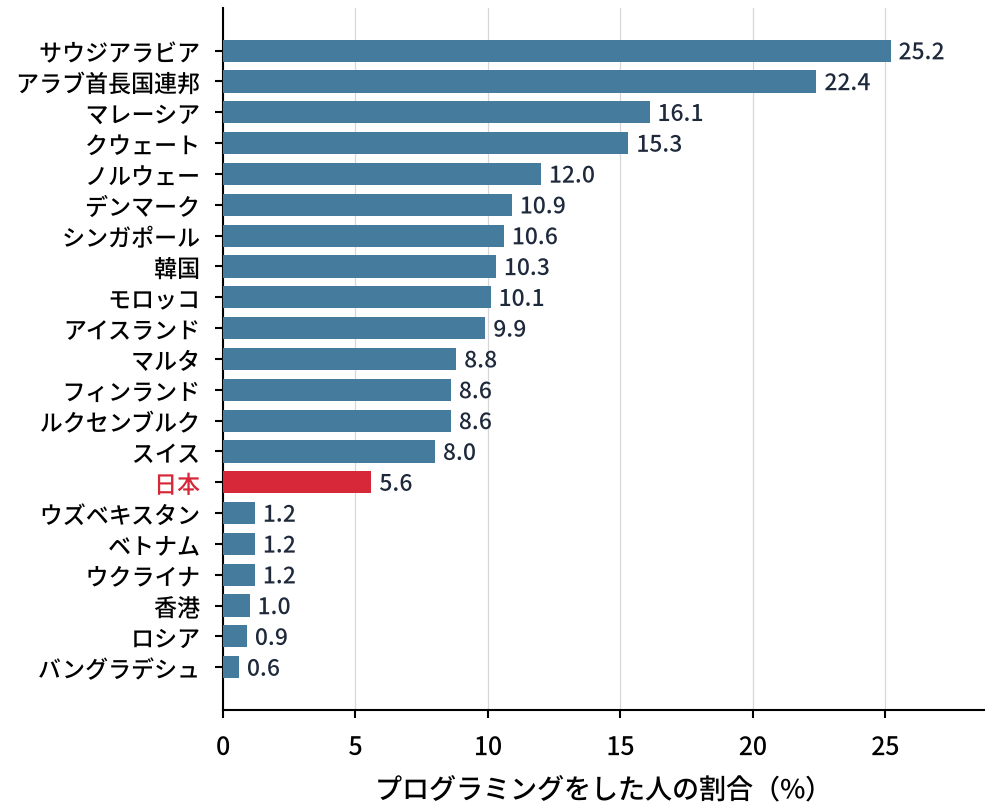
\includegraphics[width=\columnwidth]{chart_unesco_world_ict_skills.png}\caption{プログラミングをした人の割合の値の比較（上位・下位と日本を抜粋）．赤が日本}\end{figure}
\begin{figure}[t]\centering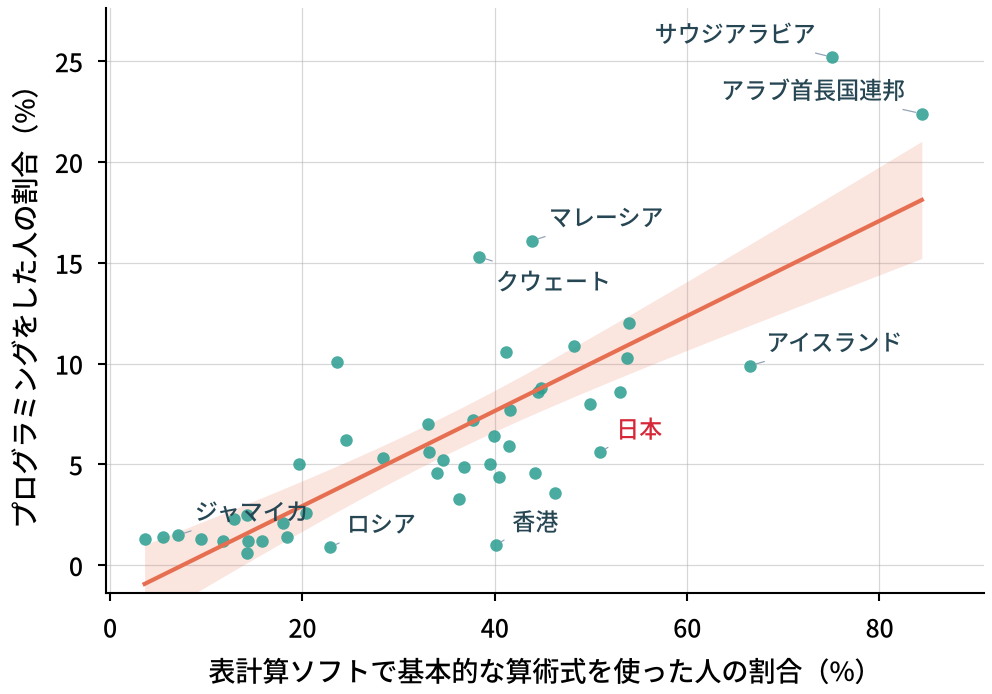
\includegraphics[width=\columnwidth]{chart_secondary_unesco_world_ict_skills.png}\caption{表計算ソフトで基本的な算術式を使った人の割合とプログラミングをした人の割合の関連（回帰直線と，その平均の95\%信頼区間の帯，n=47）}\end{figure}
\begin{table}[t]
\caption{プログラミングをした人の割合を従属変数とした重回帰分析}
\centering\scriptsize\setlength{\tabcolsep}{3pt}
\begin{tabular}{>{\raggedright\arraybackslash}p{3.0cm}rrrr}
\toprule
説明変数 & $\beta$ & 95\%CI & \textit{p} & VIF \\
\midrule
表計算 & $+$0.54 & [$-$0.15, $+$0.90] & 0.015 & 4.28 \\
プレゼン資料作成 & $+$0.34 & [$-$0.00, $+$0.67] & 0.127 & 4.71 \\
表計算の男女差（男性−女性，\%ポイント） & $-$0.11 & [$-$0.39, $+$0.24] & 0.379 & 1.38 \\
\bottomrule
\end{tabular}
\par\smallskip{\scriptsize 注）従属変数：プログラミングをした人の割合．\textit{n}=38，\textit{R}\textsuperscript{2}=0.65（調整済み 0.62），\textit{F}(3,34)=21.07．標準化係数．95\%CIはブートストラップ（2000回）．}
\end{table}
\begin{table}[t]
\caption{パス解析：直接・間接・総合の関連（標準化）}
\centering\scriptsize\setlength{\tabcolsep}{3pt}
\begin{tabular}{>{\raggedright\arraybackslash}p{3.4cm}rrr}
\toprule
経路 & 直接 & 間接 [95\%CI] & 総合 \\
\midrule
表計算 → プログラミング & 0.51 & 0.28 [0.00, 0.69] & 0.79 \\
\bottomrule
\end{tabular}
\par\smallskip{\scriptsize 注）間接の95\%CIはブートストラップ（2000回）．「直接」が0.00の経路は，モデルに含めていない．}
\end{table}
\begin{figure*}[t]\centering
\begin{tikzpicture}[>=stealth,node distance=1cm,
  obs/.style={draw,rounded corners=2pt,minimum height=1.0cm,text width=3.8cm,align=center,font=\footnotesize},
  lat/.style={draw,ellipse,minimum height=1.0cm,text width=3.4cm,align=center,font=\footnotesize},
  lab/.style={font=\scriptsize,fill=white,inner sep=1pt}]
  \node[obs] (n1917207746) at (1.40,0.00) {表計算};
  \node[obs] (n968579628) at (6.27,0.00) {プレゼン資料作成\\{\scriptsize $R^2$=.79}};
  \node[obs] (n2687051415) at (11.13,0.00) {プログラミング\\{\scriptsize $R^2$=.65}};
  \draw[->] (n1917207746) -- node[lab,pos=0.5] {.89***} (n968579628);
  \draw[->] (n1917207746.north) to[bend left=38] node[lab,pos=0.5] {.51*} (n2687051415.north);
  \draw[->,dashed] (n968579628) -- node[lab,pos=0.5] {.32} (n2687051415);
\end{tikzpicture}
\caption{パス図（標準化係数。破線は \textit{p}$\ge$.05。\textit{n}=47）}
\end{figure*}
\begin{figure*}[t]\centering
\begin{tikzpicture}[>=stealth,
  obs/.style={draw,rounded corners=2pt,minimum height=0.9cm,text width=2.33cm,align=center,font=\tiny,inner sep=2pt},
  lat/.style={draw,ellipse,minimum height=1.2cm,text width=3.27cm,align=center,font=\footnotesize,inner sep=1pt},
  lab/.style={font=\scriptsize,fill=white,inner sep=1pt}]
  \node[lat] (n4099992217) at (5.17,0.00) {オフィススキルの普及};
  \node[obs,text width=4.82cm,font=\scriptsize] (n2687051415) at (12.92,0.00) {プログラミング};
  \node[obs] (n570297867) at (1.29,-2.2) {表計算（女性）};
  \draw[->] (n4099992217) -- node[lab,pos=0.62] {.97} (n570297867);
  \node[obs] (n2132308174) at (3.88,-2.2) {表計算（男性）};
  \draw[->] (n4099992217) -- node[lab,pos=0.62] {.98} (n2132308174);
  \node[obs] (n2976367067) at (6.46,-2.2) {プレゼン（女性）};
  \draw[->] (n4099992217) -- node[lab,pos=0.62] {.90} (n2976367067);
  \node[obs] (n4018257694) at (9.04,-2.2) {プレゼン（男性）};
  \draw[->] (n4099992217) -- node[lab,pos=0.62] {.90} (n4018257694);
  \draw[->] (n4099992217) -- node[lab,pos=0.5] {.80***} (n2687051415);
\end{tikzpicture}
\caption{潜在変数を含むSEM（1因子）（標準化推定値。\textit{$\chi^2$}(5)=62.87，CFI=0.80，RMSEA=0.57，\textit{n}=36。破線は \textit{p}$\ge$.05）}
\end{figure*}
\section{考察}
RQ1では，3つの活動の割合が国・地域によって大きく異なり，日本は表計算で7番目，プログラミングとプレゼン資料作成で21番目だった．表計算とプレゼン資料作成は平均より高く，プログラミングは平均よりやや低く中央値よりやや高い．RQ2では，表計算の割合が高い国・地域ほどプログラミングの割合も高く（\textit{r}=.79），上位2か国を除いても（\textit{r}=.70），1か国ずつ除いても（\textit{r}=.74〜.81）変わらなかった．ただしプレゼン資料作成との相関（\textit{r}=.77）と差があるとは言えず，重回帰の表計算の係数は信頼区間が0を含み，パス解析の直接の関連も信頼区間が0に接し，SEMは適合がよくなかった．3つの活動がそろって高い国・地域がある，という程度に読むのが慎重で，表計算がプログラミングを高めるとは言えない．

3つの活動がそろう傾向は，デジタル資本のように複数の資源が重なるという見方（Ragnedda，2018）と整合しうる．日本は表計算から見込まれるよりプログラミングが低い側にある．デジタル格差を利用の違いとして見る議論（Selwyn，2004；Van Deursen and Van Dijk，2014）は個人間の違いが中心で，国別の集計値から検証できるものではない．Hargittai (2002)が扱ったスキルの違いやVan Dijk (2020)の議論を検討するには，頻度や質の測定が要るが，本研究の指標は「した」かどうかの自己申告である．プログラミングをした割合は，Wing (2006)の計算論的思考を測るものとは言えない．関連の理由として，活動が同じ環境や機会で身につくことが考えられるが，仮説にとどまり，本研究のデータでは検証できない．

限界は，(1)集計値のみで個人の因果を特定できないこと（生態学的誤謬），(2)自己申告で，ITUが各国の調査から集めた元の統計は調査の設計や対象年齢が国により異なること，(3)47の国・地域は欧州・中東・中南米・アジアが中心でアフリカやオセアニアは少なく，日本のプログラミングの男女別の値がないこと，(4)経済水準や通信環境などの交絡を統制していないこと，(5)2021年の1時点であること，(6)規模の小さい国・地域を除く確認をしていないこと，(7)3つのモデルは観測数が少ない探索的な当てはめで，3つの割合の分母が全成人なら，r=.79は技能の関連より機器や回線の普及を反映しうることであること，である．教育現場でこれらの活動を促す取り組みの効果は，確かめられていない．UNESCO (2023)が問うように，何のためにどの条件で技術を教育で使うかの検討は別に必要である．
\section*{参考文献}
\begingroup\scriptsize\raggedright\interlinepenalty=10000 
\begin{list}{}{\setlength{\leftmargin}{1.5\zw}\setlength{\itemindent}{-1.5\zw}\setlength{\labelwidth}{0pt}\setlength{\labelsep}{0pt}\setlength{\itemsep}{1pt}\setlength{\parsep}{0pt}\setlength{\topsep}{0pt}\setlength{\listparindent}{0pt}}
\item HARGITTAI, E. (2002) Second-level digital divide: Differences in people's online skills. First Monday, \textbf{7} (4).
\item ITU (2023) Measuring digital development: Facts and figures 2023. International Telecommunication Union, Geneva.
\item RAGNEDDA, M. (2018) Conceptualizing digital capital. Telematics and Informatics, \textbf{35} (8) ：2366-2375.
\item SELWYN, N. (2004) Reconsidering political and popular understandings of the digital divide. New Media \& Society, \textbf{6} (3) ：341-362.
\item UNESCO (2023) Global Education Monitoring Report 2023: Technology in Education - A Tool on Whose Terms? UNESCO Publishing, Paris. DOI: 10.54676/aatw1274
\item VAN DEURSEN, A. J. A. M. and VAN DIJK, J. A. G. M. (2014) The digital divide shifts to differences in usage. New Media \& Society, \textbf{16} (3) ：507-526.
\item VAN DIJK, J. (2020) The digital divide. Polity Press, Cambridge.
\item WING, J. M. (2006) Computational thinking. Communications of the ACM, \textbf{49} (3) ：33-35.
\end{list}\endgroup
\section*{Summary}
{\footnotesize\setlength{\parindent}{0pt}Using 2021 UNESCO Institute for Statistics values (originally from ITU), we compared the share of adults who reported programming, using spreadsheet formulas, and creating presentations across 47 countries and regions. Japan ranked 21st in programming (5.6\%, tied with Slovenia), 7th in spreadsheets (50.9\%), and 21st in presentations (33.5\%); means are unweighted averages across countries. Programming and spreadsheet shares were strongly correlated (r = .79, 95\% CI [0.65, 0.88], n = 47), and r remained .70 after removing the top two countries. This did not differ detectably from the correlation with presentations (r = .77), and in a multiple regression the bootstrap interval for the spreadsheet coefficient included zero. These are country-level aggregates and do not imply causation for individual adults.\par\smallskip KEYWORDS: UNESCO, ICT Skills, International Comparison, Programming, Spreadsheets\par}
\medskip\noindent\fbox{\parbox{\dimexpr\columnwidth-2\fboxsep-2\fboxrule}{\footnotesize\gtfamily 【付記：生成AIによる自動執筆に関する開示】\\ 本論文は学生への教育目的で作成している．使用しているデータは公的オープンデータである．統計の算出はPythonで行い，文章は生成AI（Anthropic Claude等）を活用して作成した．記載した統計数値は元データに準拠しているが，教育学的な考察や提言の妥当性は，指導現場の実情に応じて，批判的に吟味してほしい．}}
\end{document}
